\documentclass[conference]{IEEEtran}
\IEEEoverridecommandlockouts
% The preceding line is only needed to identify funding in the first footnote. If that is unneeded, please comment it out.
\usepackage{cite}
\usepackage{amsmath,amssymb,amsfonts}
\usepackage{algorithmic}
\usepackage{graphicx}
\usepackage{minted}
\usepackage{textcomp}
\usepackage{xcolor}
\usepackage{hyperref}
\usepackage{tabularx}
\def\BibTeX{{\rm B\kern-.05em{\sc i\kern-.025em b}\kern-.08em
    T\kern-.1667em\lower.7ex\hbox{E}\kern-.125emX}}
\begin{document}

\title{Voice assistants in hospital triage operations}

\author{\IEEEauthorblockN{Montali Simone}
    \IEEEauthorblockA{\textit{Dipartimento di Ingegneria e Architettura} \\
        \textit{Università di Parma}\\
        Parma, Italy \\
        simone.montali1@studenti.unipr.it}
    \and
    \IEEEauthorblockN{Mordonini Monica}
    \IEEEauthorblockA{\textit{Dipartimento di Ingegneria e Architettura} \\
        \textit{Università di Parma}\\
        Parma, Italy \\
        monica.mordonini@unipr.it}
    \and
    \IEEEauthorblockN{Tomaiuolo Michele}
    \IEEEauthorblockA{\textit{Dipartimento di Ingegneria e Architettura} \\
        \textit{Università di Parma}\\
        Parma, Italy \\
        michele.tomaiuolo@unipr.it}
}

\maketitle

\begin{abstract}
    This paper analyzes the creation and usage of a voice assistant for the triage of emergency room patients. This human-centred intelligent system strongly relies on Mycroft, an extensible open source voice assistant. The patients are able to declare their symptoms to the agent, which recognizes the urgency and acts accordingly. The software can even provide useful medical informations to the users.
\end{abstract}

\begin{IEEEkeywords}
    voice assistant, mycroft, hospital, er, emergency, triage
\end{IEEEkeywords}

\section{Introduction}
While the medical research progressed heavily in the last years, the involved IT infrastructures didn't. This was probably caused by the need of having ultra-reliable software, since no errors are permitted in ER rooms. The use cases of agents in hospitals are numerous. This paper inspects the automation of the triage procedures, usually done by nurses, to help patients faster and more efficiently. The voice assistant is an agent able to connect to Mycroft's cloud services, recognize the patients' symptoms and assign them a priority. It also features a second classifier, based on a deep learning network, trained on a dataset composed of ER rooms interviews. This second classifier is used every time the first one isn't capable of recognizing the symptoms. The intelligent system is even capable of interacting with the italian health ministery's website to retrieve the informations requested by the users. The triage operations produce reports in a standard format, making the integration with existing systems easy, cheap and fast. This article is composed as follows:
\begin{itemize}
    \item Section \ref{sec:voice-assistants-and-triage} introduces this project's context
    \item Section \ref{sec:mycroft} presents the Mycroft project and its peculiarities
    \item Section \ref{sec:skill-creation} describes the creation of the first module of this project
    \item Section \ref{sec:fallback} illustrates the workings of the second classifier
    \item Section \ref{sec:information-retrieval} describes the retrieval and conveying of medical informations and tips
    \item Section \ref{sec:applicability} describes this project's applicability and requirements
\end{itemize}

\section{Voice Assistants and Triage}
\label{sec:voice-assistants-and-triage}
\subsection{Voice Assistants}
Voice assistants are agents capable of interpreting human dialogs and reply through synthetized voices. The most famous examples are Amazon Alexa, Apple Siri, Google Assistant\dots The assistant waits for a \textit{wake word}, hears the request, transforms it into text, interprets it and \textit{speaks} a reply through a TTS engine. Voice assistants are rarely used in hospitals, but a report from \textbf{Voicebot} \cite{voicebot}, an organization supporting the spread of these technologies, stated that while just 7.5\% of the interviewed people had used a voice assistant in healthcare, 52\% would like to do so. Surprisingly, this includes even the higher age groups.
\subsection{Triage}
Triage is the process in which the patients requesting help in the ER are catalogued by their urgency and their priority \cite{bazyar2020principle}. The term was born during wars and maxi-emergencies, but similar operations are done everyday, in hospitals all around the world. The most famous \textit{methods} are the \textbf{START} and the \textbf{CESIRA}. The italian health ministery never defined a standard, but generally the patients get divided in 4 groups: red(critical, immediate access), yellow (life threatening, access within 15 minutes), green(access within 60-90 minutes), white. The triage produces a report containing the patient's anagraphic data, the symptoms, the urgency, date and time of access to the hospital.
\subsection{Triage and COVID19}
\label{COVID}
The COVID19 global pandemic changed the triage procedures heavily: the key is keeping patients with COVID19-compatible symptoms far from the other ones\cite{10.1093/jamia/ocaa01}. Usually, this involves the building of \textit{pre-triage} tents, where patients get tested. Integrating a fast COVID19 diagnostic in the agent could reduce the risk of infections.
\section{Mycroft}
\label{sec:mycroft}
\subsection{Why Mycroft?}
The most popular voice assistants, like Google Assistant or Amazon Alexa, are proprietary software made by corporations. While this may be good for the usability and functionality, it lacks a critical feature: privacy. Since trust, security and privacy of health data are tremendously precious, we need to protect them, and doing that while using a proprietary voice assistant is kind of impossible. Choosing an open source alternative allows us to guarantee \textbf{data privacy}, \textbf{extensibility}, \textbf{customizability}, and last but not least, \textbf{a free tool that every hospital could use}.
\subsection{The Mycroft project}
Mycroft was born to provide an open source voice assistant to users, developers, researchers.\cite{mycroft} It was initially funded with a crowdfunding in 2015, and obtained great success. The project is based on a subset of tools built by Mycroft, Inc and other companies:
\begin{itemize}
    \item Precise, a wake word listener based on a \textit{Gated Recurring Unit}, a recurrent neural network similar to an LSTM with a forget gate \cite{GRU}. It is trained over audio tracks, not text, making the software compatible with different accents, dialects, languages.
    \item The Speech To Text component isn't enough stable yet. Because of this, this project uses the Google STT engine \cite{google-stt}. The requests are bucketed and proxied through Mycroft's servers to provide a privacy layer.
    \item The intent interpretation is based on two tools: \textbf{Padatious} and \textbf{Adapt}. While Adapt is based on keywords recognition, Padatious is based on a neural network trained over full phrases. Padatious can even extract entities from the intent, like a city name or a disease.
    \item While Mycroft built a Text To Speech engine, \textbf{Mimic}, it isn't currently available in italian. Because of this, we're using the Google STT engine, with proxied requests.
    \item A graphical user interface was built over the Qt library using KDE Plasmoids, graphical components available in the KDE Plasma desktop environment.
\end{itemize}
\section{Skill Creation}
\label{sec:skill-creation}
The greatest power Mycroft has to offer is its modularity: every responsibility is tied to a single module, named \textbf{skill}, which interprets the related requests and provides an answer. Some examples might be a joke-telling skill, a reminder skill, a timer skill. When Mycroft receives a request, it checks all of the skills' intents for matches. If a match is found, the related function is called.
Skills are coded in Python, and have a standard structure. To generate the boilerplate code for a new skill, Mycroft provides a command line interface.
\subsection{Skills file structure}
Skills have a standard file structure and file types:
\begin{itemize}
    \item \texttt{dialog} files: these files contain the assistants's answer dialogs. Multiple phrases are included and randomly chosen: this makes the assistant more \textit{human}.
    \item \texttt{intent} files: these files are used to train the Padatious' neural network. They contain example phrases for every intent.
    \item \texttt{voc} files: these files contain Adapt keywords. Since this project strictly relies on Padatious, these are almost not used.
    \item \texttt{entity} files: these files contain entities to be extracted by padatious, like city names, diseases\dots
    \item \texttt{settingsmeta.yaml}: this YAML file defines the skill's settings, to be edited on the Mycroft Home website.
    \item \texttt{\_\_init\_\_.py}: this file contains the skill's main code. It is based on an extension of the \texttt{MycroftSkill} class, which contains the classes and decorators needed to define a new skill.
\end{itemize}
\subsection{hospital-triage-skill}
The skill is structured as follows: every symptom type is caught in an intent. Basing on the symptom type, different things happen: a urgency code is assigned to the patient (red, yellow, green), anagraphical data is collected, minor symptoms are checked\dots
All the collected data gets saved to a Python dictionary to be exported in JSON. All the \textit{standard} operations, like asking for a pain evaluation or the patient's name, are handled by decorators.
\subsection{The \texttt{covid\_symptom} decorator}
The COVID19 global pandemic strongly changed how people behave, interact, get cured. As already discussed in section \ref{COVID}, hospitals need to keep COVID19-compatible patients separate from the other ones, and from each other. Automating the COVID19 diagnostic may be crucial now. Therefore, the voice assistant needs to check if the patient may be infected and potentially contagious.
Because of this, all of the symptoms that are slightly connected with COVID19 trigger a diagnostic handled by the \texttt{covid\_symptom} decorator.
This asks the patient for known symptoms\cite{paginemediche}, and multiplies a score (by default equal to $1$) by their \textit{multiplier}:
\begin{itemize}
    \item \textbf{Fever}: multiplied by $2.0$
    \item \textbf{Sore throat}: multiplied by $1.3$
    \item \textbf{Cold}: multiplied by $1.3$
    \item \textbf{Breathing fatigue}: multiplied by $1.6$
    \item \textbf{Cough}: multiplied by $1.6$
    \item \textbf{Contact with infected people}: multiplied by $3.0$
    \item \textbf{Missing sense of taste}: multiplied by $1.7$
\end{itemize}
Every suspected patient starts with a score of $1$, and if the final score reaches a threshold (by default equal to 15, but it can be adjusted basing on the pandemic's recession) the patient is advised to stay where he is and wait for a doctor to visit him.
\subsection{Helpers}
The agent needed some helpers to cope with challenges the italian language implies. An example might be the temperature extraction from an utterance: some inputs may be \textit{"trentasette e mezzo", "trentasette punto cinque", "trentasette virgola cinque", "trentasette cinque"}, \textbf{all meaning the same thing}. Another example is the number validation: the bot may interpret a "sei" as the verb \textit{essere} instead of a number.
\subsection{The exported data}
All of the collected and infered data gets exported to a JSON file. Using a standard like JSON makes integrating the bot with existing systems easy: the hospitals don't need to entirely change their informative systems, they just need to integrate some small components. An example of triage report of a COVID19 infected patient may be the following:
\begin{minted}{json}
{
    "can_talk": "yes",
    "main_symptom": "breathing",
    "code": "red",
    "fever": 38.7,
    "has_sore_throat": "yes",
    "has_cold": "no", 
    "has_breathing_difficulties": "yes", 
    "has_cough": "yes",
    "has_had_contacts": "yes",
    "misses_taste": "yes",
    "covid_score": 22.6304,
    "symptom_declaration": "ho il fiatone",
    "age": 21,
    "other_symptoms": "ho mal di testa", 
    "pain_index": "8",
    "full_name": "marco rossi"
}
\end{minted}
\subsection{Conversation example}
A conversation with the bot may be the following:
\begin{itemize}
    \item \textbf{User}: \textit{Can you help me?}
    \item \textbf{Voice assistant}: \textit{Are you the one seeking medical treatment?}
    \item \textbf{User}: \textit{Yup.}
    \item \textbf{Voice assistant}: \textit{What is your main symptom?}
    \item \textbf{User}: \textit{I have a fever.}
    \item \textbf{Voice assistant}: \textit{Ok, a fever. Have you measured it recently?}
    \item \textbf{User}: \textit{Yes.}
    \item \textbf{Voice assistant}: \textit{Please, tell me your temperature.}
    \item \textbf{User}: \textit{Thirtyseven point eight.}
    \item \textbf{Voice assistant}: \textit{I need some additional informations for the diagnosis. I will now ask you some yes/no questions. Do you have a sore throat?}
    \item \textbf{User}: \textit{Yes.}
    \item \textbf{Voice assistant}: \textit{Do you have a cold?}
    \item \textbf{User}: \textit{Yes.}
    \item \textbf{Voice assistant}: \textit{Do you have any trouble breathing?}
    \item \textbf{User}: \textit{No.}
    \item \textbf{Voice assistant}: \textit{Do you have a cough?}
    \item \textbf{User}: \textit{Yes.}
    \item \textbf{Voice assistant}: \textit{Have you been in contact with people infected by the new coronavirus?}
    \item \textbf{User}: \textit{Yes.}
    \item \textbf{Voice assistant}: \textit{We're notifying a doctor. It is possible that you may be infected by COVID19. Could you tell me how old you are?}
    \item \textbf{User}: \textit{Twentytwo.}
    \item \textbf{Voice assistant}: \textit{How would you define your discomfort from 1 to 10?}
    \item \textbf{User}: \textit{Eight.}
    \item \textbf{Voice assistant}: \textit{If there's any other symptoms I need to know, please tell me}
    \item \textbf{User}: \textit{Nothing else.}
    \item \textbf{Voice assistant}: \textit{Could you please tell me your full name?}
    \item \textbf{User}: \textit{Simone Montali.}
    \item \textbf{Voice assistant}: \textit{Simone Montali, is that right?}
    \item \textbf{User}: \textit{Yes.}
    \item \textbf{Voice assistant}: \textit{Thanks for your patience, go at the RED desk.}
\end{itemize}
\section{Fallback skills and NLP}
\label{sec:fallback}
A problem now arises: what if the patient has a disease which was not covered in the previous symptoms? The intent would not be caught. Sadly, diseases are so vast and numerous that it would be impossible to hardcode them: we need a \textit{statistical} approach. The target is now building a text classifier that is able to classify the patient's declaration to a symptomatology or at least an hospital ward.
\subsection{Dataset}
Since the medical data is fortunately well protected by privacy laws all around the world, finding medical datasets is not easy. However, creating a dataset from scratch is still possible: this is exactly what \textbf{Appen}, an australian start up, did. The dataset used in this project \cite{dataset} contains audio snippets, transcriptions and symptomatologies of patients requesting help to nurses. Since the Mycroft's STT engine handles the conversion to text, we only need to train a classifier that maps patient requests to symptom types. An example of this dataset's entries may be:
\begin{itemize}
    \item \textbf{Phrase}: \textit{My son had his lip pierced and it is swollen and the skin inside
              on his lip is grey and looks infected.}
    \item \textbf{Prompt}: \textit{Infected wound}
\end{itemize}
\subsection{Dataset translation}
Since the voice assistant was mainly born for italian users, we need to translate the dataset to italian. Using Google Translate's APIs would be easy but costly. We could use a scraper to query Google Translate's webpage, but that would be slow. Fortunately, third party Python modules have been made: \texttt{googletrans} is the most famous. Using it, we were able to translate the dataset with a simple script.
\begin{minted}[]{python}
for index, row in data.iterrows():
    phrase = translator.translate(
        row["phrase"], 
        dest="it").text
    prompt = translator.translate(
        row["prompt"],
        dest="it").text
    if translator.detect(phrase).lang == "it"
     and translator.detect(prompt).lang == "it":
        translated_data.at[i, "phrase"] = phrase 
        translated_data.at[i, "prompt"] = prompt 
        i = i+1
\end{minted}
When Google Translate can't recognize a phrase's meaning, it skips it. The \texttt{translator} object, besides translating things, can even detect languages. This allows us to do a little workaround: if the detected language isn't italian in both the phrase and the symptomatology, the entry is skipped. This reduced the dataset from 8000 entries to almost 2000.
\subsection{Classifier training}
Having an italian dataset, we can now proceed with the classifier's training. To do so, using the \textbf{fastai} library simplifies things: it provides the \texttt{text.learner} class, which is able to train a model and export it. This enables us to train the model a single time, and simply import it into the voice assistant.
\subsection{Data preparation and training}
We can now import our dataset in a Jupyter notebook, check for NaNs, and create the \texttt{text.learner} with fastai. For the project, we used the AWD-LSTM structure, a recurrent neural network which has really high performance on text processing. This type of network has a \textbf{Long Short Term Memory}\cite{lstm}, which enables the training to find patterns in distant parts of the text, \textbf{Average SGD} and \textbf{Dropconnect}, a dropout that drops weights instead of activations \cite{awd-lstm}. We can now train the network and check the confusion matrix:
\begin{figure}[H]
    \begin{center}
        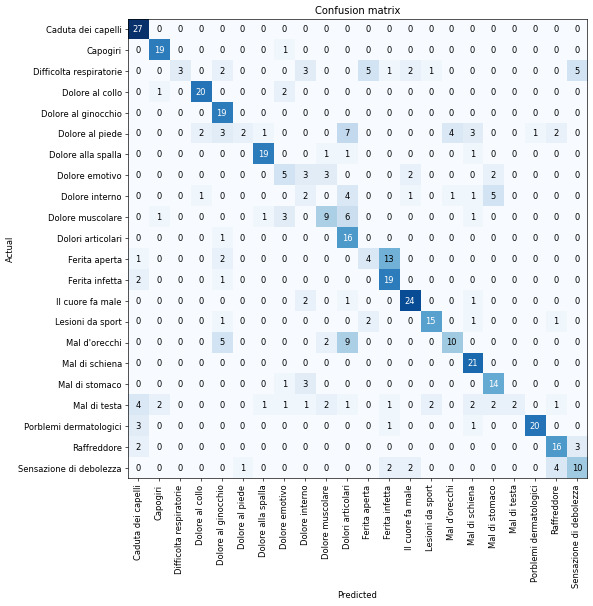
\includegraphics[width=\columnwidth]{ConfusionMatrix.jpg}
    \end{center}
    \caption{Confusion Matrix}
    \label{fig:confusion-matrix}
\end{figure}
While it isn't perfect, the diagonal in the matrix shows that \textbf{the model was trained correctly}. Talking about accuracy, the model reached \textbf{more than 60\%}:
\begin{figure}[H]
    \begin{center}
        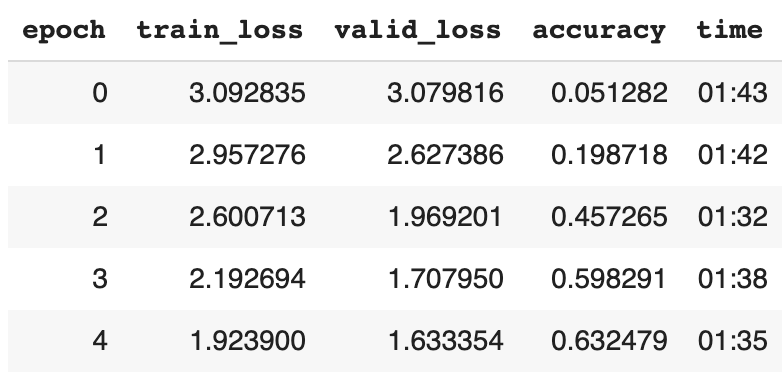
\includegraphics[width=\columnwidth]{Accuracy.png}
    \end{center}
    \caption{Accuracy}
    \label{fig:accuracy}
\end{figure}
We can now easily export it and integrate it in the voice assistant by a simple import.
\subsection{Fallback skills creation}
As explained earlier, Mycroft works by recognizing intents in the user's requests. These were defined in the last skill, but the symptomatologies are more than the ones coded. However, Mycroft makes it possible to define \textbf{fallback skills}, a skill that gets triggered every time the intent is not recognized. By creating one, we're able to get the patient's utterance and analyze it with our classifier. Fallback skills are ordered by a priority, but since our voice assistant will have just one, it doesn't matter. After registering the fallback skill, we can import the model. The symptomatologies inserted in the model are defined in a separate \texttt{classes.json} file, containing each symptom's urgency, GUI emoji, name, and its compatibility with COVID19. An example would be:
\begin{minted}[]{json}
{
    "name": "Dolore al collo",
    "emoji": "[removed]",
    "code": "yellow",
    "covid": false
}
\end{minted}
Having done that, the symptoms can now be handled like any other one. Ideally, we'd like to check if the classifier worked right by asking the patient.
An example of conversation may be:
\begin{itemize}
    \item \textbf{User}: \textit{I need help.}
    \item \textbf{Voice assistant}: \textit{Are you the one seeking medical treatment?}
    \item \textbf{User}: \textit{Yes.}
    \item \textbf{Voice assistant}: \textit{What is your main symptom?}
    \item \textbf{User}: \textit{My shoulder dislocated while I was playing golf.}
    \item \textbf{Voice assistant}: \textit{So, we're talking about shoulder pains, right?}
    \item \textbf{User}: \textit{Yes.}
    \item \textbf{Voice assistant}: \textit{Could you tell me how old you are?}
    \item \textbf{User}: \textit{Twenty.}
    \item \textbf{Voice assistant}: \textit{How would you define your pain from 1 to 10?}
    \item \textbf{User}: \textit{Nine.}
    \item \textbf{Voice assistant}: \textit{If there's any other symptoms I need to know, please tell me}
    \item \textbf{User}: \textit{Nothing else.}
    \item \textbf{Voice assistant}: \textit{Could you please tell me your full name?}
    \item \textbf{User}: \textit{Mario Rossi.}
    \item \textbf{Voice assistant}: \textit{Mario Rossi, is that right?}
    \item \textbf{User}: \textit{Yes.}
    \item \textbf{Voice assistant}: \textit{Thanks for your patience, go at the YELLOW desk.}
\end{itemize}
\section{Information retrieval}
\label{sec:information-retrieval}
This agents's use cases might not be limited to triage and helping in emergencies. In fact, a patient could just want to know some medical informations about a particular disease without having to talk to a doctor.
\subsection{Data source}
It is obvious that the data source we're looking for has to be authoritative: Wikipedia is not reliable enough. Luckily, the italian health ministery published a medical encyclopedia on their website. These informations are complete, reliable and interesting. To be able to use them, we can scrape the website using tools like \textbf{Selenium}. Selenium is a framework used to test web applications; it provides a simple interface to automate a web browser\cite{selenium}. We could use two approaches for the data collection: an API approach, which downloads the informations basing on queries, or a periodic one. The first one is possible thanks to the Python \texttt{http.server} library, in which we can define a handler for GET requests. This will look for the query on the encyclopedia, download the page, insert the data into a JSON and return it. Since the informations on the website rarely vary, we can download them periodically and keep them saved. By defining a script that iterates over every item in the encyclopedia, we can download all the needed informations. Using \textbf{cron}, a job scheduler for Linux, it's possible to automatically download the data periodically.
\subsection{Integration of the data into the voice assistant}
Having the data, we can now define a new intent in the voice assistant to request informations. Padatious' entity extraction simplifies this: we can train it with phrases like \textit{"Tell me something about \{disease\}"}, creating a \textit{disease} entity containing all the known diseases. These are not strictly exact matches: we're looking for the best match, so that if the user asks something about \textit{tumor in the lung}, \textit{lung tumor} is matched. After matching the name, the assistant checks the known data, like \textit{prevention, cure, therapy, symptoms}, and asks the patient to choose.
An example of conversation might be the following:
\begin{itemize}
    \item \textbf{User}: \textit{What do you know about celiac disease?}
    \item \textbf{Voice assistant}: \textit{The best match is celiac condition, is that what you're looking for?}
    \item \textbf{User}: \textit{Yes.}
    \item \textbf{Voice assistant}: \textit{What would you like to know? Choose between Description, Symptoms, Causes, Therapy, Complications}
    \item \textbf{User}: \textit{Tell me the causes.}
    \item \textbf{Voice assistant}: \textit{This is what I know: celiac disease is a multifactorial condition\dots}
\end{itemize}
\section{Applicability and technical requirements}
\label{sec:applicability}
Since this agent could enhance the hospitals' workflow all around the world, it has built to be as cheap and easy as possible. The TTS and STT engines are computed in cloud: this removes the most computationally heavy module from our responsibility. The intent parser, Padatious, needs an ultra light training just once every start of the bot. Even if the computer is not powerful, it requires just a few minutes. The fastai training is computed in cloud: the model gets exported and used without any further training. This doesn't require any computational power. The only real requirement is defined by the GUI: since it is built on KDE Plasmoids, the desktop environment has to be KDE Plasma. Mycroft recommends using KDE Neon, a Ubuntu LTS distribution with KDE Plasma installed. The devices that support this project are, therefore, almost infinite: even a simple Raspberry Pi or an old computer can run Mycroft.
\section{Conclusions}
\label{sec:conclusions}
The global pandemic the world had to bear with has highlighted how hospitals, in the last years, have been forgotten by politicians, people, nations. In the last 20 years, in Italy, the number of institutes diminished from 311 thousands to 191 thousands, while the public spending was raised from 60 miliards to 112\cite{ospedali-agi}. With the aid of human-centred intelligent systems, health workers could get some relief and concentrate on what matters more: curing people. Voice assistants could \textit{flatten} the
\textit{digital divide}, being easy to use for everyone, including the elder. Translation of the agent to multiple languages could be an incredible tool for immigrants, tourists and travelers who can't speak the national language. Right now, the most urgent improvement to make is finding or creating a better dataset: if the classifier worked better, we could skip the hardcoding of the most common symptoms and just leave one skill. The ultra low cost of this project's requirements makes it possible for every hospital in the world to install a tool like this. The open source design (all the source code is licensed with a GPL-3.0 license) guarantees freedom, privacy, expansibility, customizability, and, last but not least, the possibility of saving lives without having to pay a price.
\section{Source code}
Every single line of code of this project is open source and available on GitHub:
\begin{itemize}
    \item Mycroft skill for the triage operations and the information requests: \href{https://github.com/montali/hospital-triage-skill}{montali/hospital-triage-skill}
    \item Fallback skill for the NLP classification and diagnosis of symptoms: \href{https://github.com/montali/hospital-fallback-skill}{montali/hospital-fallback-skill}
    \item Health Ministery's encyclopedia scraper: \href{https://github.com/montali/medical-infos-api}{montali/medical-infos-api}
\end{itemize}

\begin{thebibliography}{00}
    \bibitem{voicebot} Voicebot - Orbita, "Voice Assistant Consumer Adoption in Healthcare", In: (ott. 2019).
    \bibitem{triage} Ministero Della Salute, \href{http://www.salute.gov.it/imgs/C_17_notizie_3849_listaFile_itemName_1_file.pdf}{"Linee di indirizzo nazionali sul triage interospedaliero"},
    \bibitem{bazyar2020principle} The principles of triage in emergencies and disasters: a systematic review,Bazyar, Jafar and Farrokhi, Mehrdad and Salari, Amir and Khankeh, Hamid Reza,Prehosp Disaster Med,6,1--9,2020
    \bibitem{10.1093/jamia/ocaa01} Judson, Timothy J and Odisho, Anobel Y and Neinstein, Aaron B and Chao, Jessica and Williams, Aimee and Miller, Christopher and Moriarty, Tim and Gleason, Nathaniel and Intinarelli, Gina and Gonzales, Ralph, \href{https://doi.org/10.1093/jamia/ocaa051}{Rapid design and implementation of an integrated patient self-triage and self-scheduling tool for COVID-19},Journal of the American Medical Informatics Association,27,6,860-866,2020,05,1527-974X,10.1093/jamia/ocaa051
    \bibitem{paginemediche} Pagine Mediche, \href{https://www.paginemediche.it/coronavirus}{Nuovo Coronavirus Covid-19}
    \bibitem{mycroft} Rebecca Harrington, \href{https://www.popsci.com/ultimate-diy-ai/}{"Customize An Open-Source HAL For Your Home"}, 2016
    \bibitem{GRU} Felix Gers; Jürgen Schmidhuber; Fred Cummins (1999). "Learning to Forget: Continual Prediction with LSTM". Proc. ICANN'99, IEE, London. 1999: 850–855
    \bibitem{google-stt} Google, \href{https://cloud.google.com/speech-to-text}{Speech-To-Text}
    \bibitem{qt} Qt, \href{https://www.qt.io/}{Official website}
    \bibitem{dataset} Paul Mooney - Appen, "Medical Speech, Transcription, and Intent", 2019.
    \bibitem{fastai} fastai, \href{https://docs.fast.ai/}{Official docs}
    \bibitem{awd-lstm} Stephen Merity; Nitish Shirish Keskar; Richard Socher, Regularizing and Optimizing LSTM Language Models, 2017
    \bibitem{lstm} Sepp Hochreiter e Jürgen Schmidhuber, "Long short-term memory", In: Neural computation 9,8 (1997), pp. 1735–1780.
    \bibitem{selenium} Selenium, \href{https://github.com/SeleniumHQ/selenium}{Official repository}
    \bibitem{ospedali-agi} Agenzia Giornalistica Italia, "La riduzione di ospedali e posti letto negli ultimi 10 anni", In: (mar. 2020)
\end{thebibliography}

\end{document}
